\chapter{智能建筑领域本体}
\label{ch2}
	智能建筑是一种典型的能量信息物理融合系统(Cyber-Physical Energy System,CPES),它密切关注系统中能量的产生与消耗,且融合了复杂的物理行为和计算机网络。由于系统涉及多学科,且具有混成、随机的特点,对智能建筑进行建模、分析的第一步是明确系统中的诸多概念及它们之间的关系,从而确定研究范围,为开展后续系统设计和分析环节做准备。而领域本体能够构建领域内共同认可的概念、概念间的关系以及约束。因此,建立智能建筑的领域本体能够根据系统需求,帮助梳理系统概念和逻辑,对于开展系统的建模与分析具有必要性。基于建筑信息模型和本体构造方法的基本步骤,本章给出了智能建筑领域本体,并介绍了如何利用领域本体来指导构建系统的MARTE/UML初步模型,明确影响系统能耗的直接、间接因素,实现从需求分析到系统设计的过渡。
	
\section{智能建筑领域本体}
	1991年,人工智能领域的学者Neches等人给出本体的定义,即:本体是构成相关领域词汇的基本术语和关系,以及利用这些术语和关系构成的规定这些词汇外延规则的定义\citep{王乐2008基于本体的垂直搜索引擎研究,DBLP:journals/aim/NechesFFGPSS91}。常见的本体构造方法有骨架法、TOVE法和七步法\citep{张文秀2011领域本体的构建方法研究}等,参考这些构造方法,可总结得出本体构造的主要步骤为:1)确定领域本体的专业领域和范畴;2)考虑能否复用现有的本体;3)列出本体涉及领域中的重要术语;4)定义分类概念和概念分类层次;5)定义概念之间的关系和约束。本文针对的是智能建筑领域,重点关注智能建筑系统中的能耗。虽然暂无可复用的领域本体,但可利用建筑信息模型为本体构造提供帮助,下面,我们将按照本体构造步骤,依次给出智能建筑领域的基本术语、概念间的关系,约束和规则。
	
\subsection{基本术语}
	建筑信息模型(Building Information Model,BIM)\citep{DBLP:conf/wsc/OckIF16}是建筑物的数据信息化模型。从通用工业的角度来看,一个BIM由建筑物的所有共享数据以及物理特性、功能特性构成。BIM促进了不同的利益相关者在该建筑生命周期的各个阶段进行有效的协作,为建筑的整个生命周期的决策提供了可靠的依据\citep{张文秀2011领域本体的构建方法研究}。
	
	参考BIM对建筑物信息分类的思想,本文将智能建筑视作物理环境、建筑物和用户三部分的组合。图\ref{ontology_sb}给出了智能建筑中基本术语的概念层次图,其中,矩形表示实体概念,实线椭圆表示参数概念,虚线椭圆表示行为概念,参数和行为是依附于实体的。绿色标注的实体为直接产生或消耗能量的实体。
	\begin{figure}[!t]
	\centering
	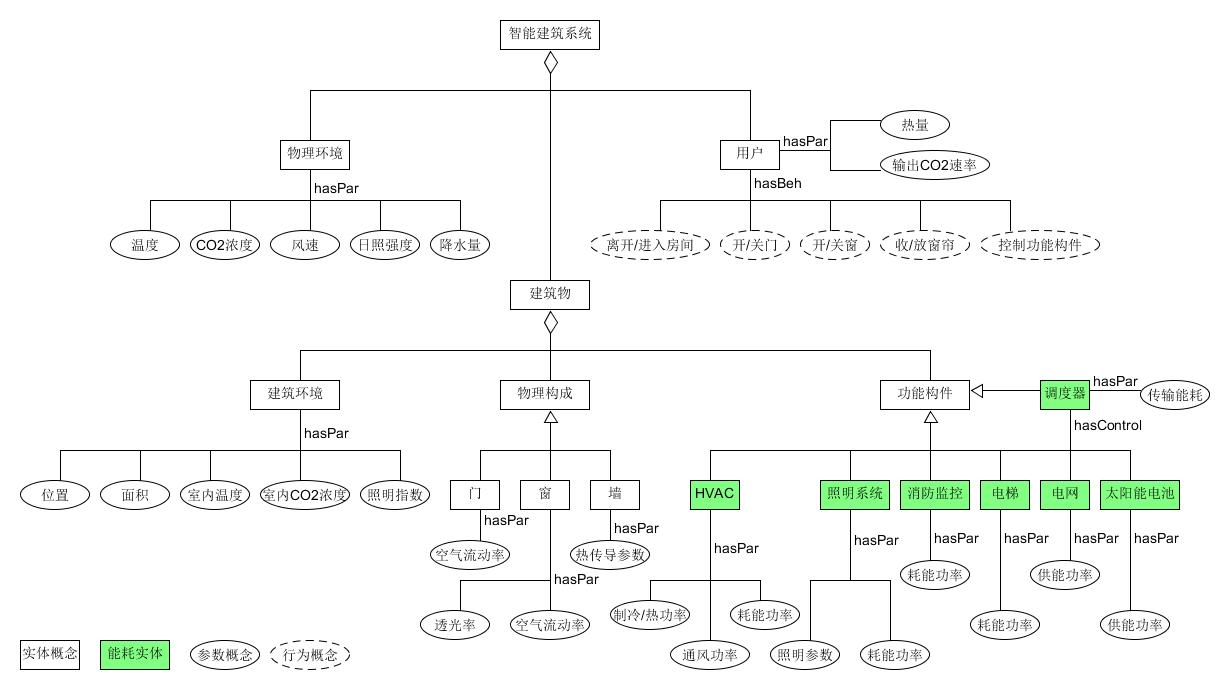
\includegraphics[width=6in]{ontology-sb-new.jpg}
	\caption{智能建筑基本术语的概念层次}
	\label{ontology_sb}
	\end{figure}
	
	\begin{itemize}
	\item \textbf{ 建筑物}:1)除了位置、面积这类基本参数外,由于智能建筑为人提供服务,建筑环境参数应包含建筑物室内环境中对人有影响的参数:$CO_{2}$浓度、室内温度,照明强度;2)物理构成则包含对上述室内参数有影响的建筑实体——门、窗和墙,这些物理构成对应有各自的具体参数;3)建筑物的功能构件是指为人类生活提供各种服务的实体,这些功能构件在使用时往往伴随着能量的产生与消耗,如太阳能电池可以将物理环境中的太阳能存储起来,为整个建筑物生产能量;而照明系统的工作会消耗一定的系统能量。功能构件也对应各自的具体参数,来表示其功能作用的影响和能耗速率。一个建筑物最基本的功能构件是暖通空调(Heating, Ventilation and Air Conditioning, HVAC)和照明系统,它们可以保证用户生存环境中最基本空气质量、温度和照明要求。调度器是一种特殊的功能构件,它负责控制其他功能构件,并且,调度器在控制其他功能构件时会传送信号,消耗系统能量。
	\item \textbf{物理环境}:对于智能建筑系统而言,系统的外部环境包括物理环境和用户。物理环境主要包含能够影响智能建筑室内环境的各种环境参数,例如,$CO_{2}$含量、温度,风速和日照强度,这些参数的取值与时间相关,其变化过程是连续的。且这些物理环境参数只能被智能建筑系统监测,不能被控制,是系统中的不可控因素。
	\item \textbf{用户}:用户存在各种行为,在此,我们考虑的是那些对系统产生影响的行为。用户行为可以触发系统的控制决策,例如在某个夏季的夜晚,用户进入房间会触发智能建筑的照明系统、暖通空调的开关;同时,用户行为也可以直接控制系统的功能构件,如开/关空调。用户自身对应的参数也会对智能建筑的室内环境造成影响\citep{Library2012American}——人体产生的热量会影响温度,$CO_{2}$的输出速率会影响室内$CO_{2}$浓度。用户行为是一种随机行为,也是系统中的不可控因素。
	\end{itemize}
	
\subsection{关系}
	智能建筑领域本体中的概念不是孤立存在的,它们之间存在各种各样的联系,这些概念以及概念间的关系构成了智能建筑的概念体系。具体来说,这些关系可分类为结构关系和交互关系。
	\begin{itemize}
	\item 结构关系:
	在图\ref{ontology_sb}中标注了不同概念之间的结构关系,参考文献\citep{陈小红2011基于问题框架的需求建模}中使用的方法,可以利用表格(表\ref{ontology_relation})详细解释这些关系。
	\item 交互关系:
	上下文图能够显式系统不同实体之间的信息交互关系,类似门、窗、墙这种物理构成,虽然它们的物理属性特征会对室内环境参数造成影响,但这些属性是恒定的,因此,只需记录这些实体的特定属性,无需在交互关系中创建对象。
	由图\ref{context}可以知道,虽然智能建筑中的功能构件是系统的主要能耗来源,但其他实体通过信息交互影响调度器对功能构件的控制,从而间接影响系统能耗。
	\end{itemize}
	
	\begin{table}[!t]
	\scriptsize
	\renewcommand{\arraystretch}{1.4}
	\caption{智能建筑领域本体概念间的结构关系}
	\label{ontology_relation}
	\centering
	\begin{tabular}{p{2cm}p{4.5cm}p{7.5cm}}
	\hline
	Association & Formation & Meaning \\
	\hline
	组合 & 物理环境、建筑物、用户 $\rightarrow$ 智能建筑系统 & 智能建筑系统由物理环境、建筑物和用户构成 \\
	hasPar & 物理环境 $\rightarrow$ 温度、$CO_{2}$浓度、风速、日照强度、降水量 & 物理环境包含的参数有温度、$CO_{2}$浓度、风速、日照强度,降水量\\
	组合 & 建筑环境、物理构成、功能构件 $\rightarrow$ 建筑物 & 建筑物由建筑环境和各种物理构成、功能构件组成\\
	hasPar & 建筑环境 $\rightarrow$ 位置、面积、室内温度、室内$CO_{2}$浓度、照明指数 & 建筑物环境包含的参数有位置、面积、室内温度、室内$CO_{2}$浓度,照明指数\\
	继承 & 门、窗、墙 $\rightarrow$ 物理构成 & 门、窗、墙都是一种具体的物理构成\\
	hasPar & 门 $\rightarrow$ 空气流动率 & 门的开/关会对室内温度和空气的流动产生影响\\
	hasPar & 窗 $\rightarrow$ 透光率、空气流动率 & 窗的开/关会对室内温度和空气的流动产生影响;窗玻璃的透光率影响了室内照明情况\\
	hasPar & 墙 $\rightarrow$ 热传导参数 & 墙的热传导参数决定了外界温度对室内温度的影响\\
	继承 & HVAC、照明系统、消防监控、电梯、电网、太阳能电池 $\rightarrow$ 功能构件 & HVAC、照明系统、消防监控、电梯、电网、太阳能电池都是一种具体的功能构件\\
	hasPar & HVAC $\rightarrow$ 制冷/热功率、通风功率、耗能功率 & HVAC系统的参数包括制冷/热功率、通风功率、耗能功率\\
	hasPar & 照明系统 $\rightarrow$ 照明参数、耗能功率 & 照明系统的参数包括照明参数、耗能功率\\
	hasPar & 消防监控/电梯 $\rightarrow$ 耗能功率 & 消防监控/电梯这类耗能构件对应的参数是耗能功率\\
	hasPar & 电网/太阳能电池 $\rightarrow$ 功能功率 & 电网/太阳能电池这类供能构件对应的参数是供能功率\\
	hasControl & 调度器 $\rightarrow$ HVAC、照明系统、消防监控、电梯、电网、太阳能电池 & 调度器可以控制其他功能构件\\
	hasPar & 调度器 $\rightarrow$ 传输能耗 & 调度器在通过信号控制其他功能构件时,会产生传输能耗\\
	hasBeh & 用户 $\rightarrow$ 离开/进入房间、开/关门、开/关窗、收/放窗帘、控制功能构件 & 用户具有的行为包括离开/进入房间、开/关门、开/关窗、收/放窗帘、控制功能构件\\
	\hline
	\end{tabular}
	\end{table}
	
	\begin{figure}[!t]
	\centering
	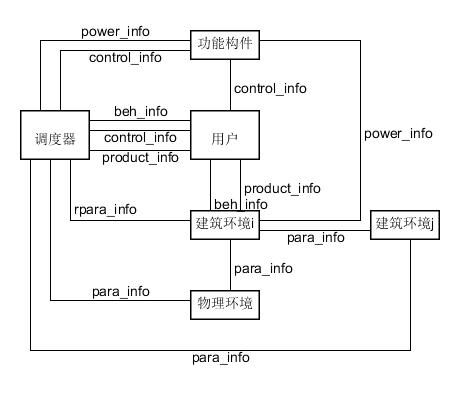
\includegraphics[width=3.8in]{context.jpg}
	\caption{智能建筑领域本体概念间的交互关系}
	\label{context}
	\end{figure}
	
\subsection{约束和规则}
	在定义了智能建筑领域本体的概念层次和概念之间关系的基础上,为了准确建模这些元素,还有必要说明某些概念之间的相互约束以及某些实体对应的规则。室内环境参数约束定义了某个具体的室内环境参数所受影响的来源,这些来源为实体的参数或实体的行为。正如上文提及,在日常场景中,对人类生活影响最大的是温度、空气质量和照明情况,下面给出关于这三个参数的约束:
	
	\textbf{室内环境参数约束}
	\begin{enumerate}
	\item 室内的$CO_{2}$浓度与物理环境$CO_{2}$浓度、用户的离开/进入房间、开/关门行为、开/关窗行为、人的$CO_{2}$输出速率、通风系统的作用以及调度器的控制有关。
	\item 室内温度与外界温度(物理环境温度和相邻空间温度)、墙的热传导性能、用户的离开/进入房间、开/关门行为、开/关窗行为、人的散热、暖通空调的作用以及调度器的控制有关。
	\item 建筑物照明指数与日照强度、窗玻璃的透光率、用户的离开/进入房间、开/关窗行为、收/放窗帘行为、照明系统的作用以及调度器的控制有关。
	\end{enumerate}

	智能建筑中的功能构件不仅可以被系统控制,也可以被人为操纵;且智能建筑中存在各种功能构件,既包括暖通空调、照明系统和电梯这些基本功能构件,也包含电视、烤箱等非基本需求的特定功能构件。下面对于功能构件的控制优先级和用能优先级给出定义。
	
	\textbf{功能构件的操作规则}
	\begin{enumerate}
	\item 控制优先级:智能建筑通过计算机网络控制系统,可实现对功能构件自动化控制。但是,当用户有特定需求时,应当可以直接控制这些构件,即用户对构件控制的优先级大于智能建筑系统控制。
	\item 构件用能优先级:系统的基本功能构件的用能优先级大于特定功能构件,当系统出现供能不足的情况时,应当优先维持对基本功能构件的供能。
	\end{enumerate}
	
\section{领域本体指导建模初步模型}
	定义智能建筑领域本体帮助我们理清了系统中的概念间的关系,也为后续的模型设计奠定了基础。下面介绍在实际建模过程中,如何利用智能建筑领域本体的概念、关系,约束和规则来指导构建MARTE/UML初步模型:
	\begin{enumerate}
	\item \textbf{选择室内环境参数}:在智能建筑领域本体概念层次图(图\ref{ontology_sb})中选择期望控制的室内环境参数。
	\item \textbf{确定相关概念}:根据室内环境参数约束,确定与选定室内环境参数相关的所有参数概念、行为概念,并将这些概念间的关系形式化为公式,可用UML参数图来记录这些公式。
	\item \textbf{构建类图}:在智能建筑领域本体概念间的关系表(表\ref{ontology_relation})中找到所有相关参数概念、行为概念依附的实体,为每个实体创建一个类,且其参数概念映射为类的属性,其行为概念映射为类的操作,并明确系统直接能耗来源的相关类;
	\item \textbf{构建顺序图}:根据上下文图中定义的不同实体概念之间的交互关系,将涉及的每个实体概念映射为对象,交互信息映射为消息事件。
	\item \textbf{构建状态图}:顺序图中的一个对象对应一个状态图,不同类型的实体概念存在各自的状态图模板:
	\begin{itemize}
	\item 物理环境:我们关心的是物理环境中的各种环境参数,这些参数的值随时间连续变化,系统只能监测这些参数,却无法控制它们,即物理环境不会由于任何系统事件的触发而改变状态。因此,在状态图中,用表达式来描述物理环境参数的变化过程。
	\item 功能构件:一个功能构件的状态图中至少包含两个状态:开启状态和关闭状态。在处于开启状态时,功能构件将根据其功率参数对系统产生影响,并且以特定的能耗功率消耗能量;在处于关闭状态时,功能构件不再耗能,也无法对系统产生任何作用。
	\item 建筑环境:建筑物的室内环境参数受到不同因素的影响,因此,应当在状态上添加对应的参数公式刻画这些因素的影响;同时,在具体的场景中,环境参数的数值可能作为判断条件触发系统的执行动作。
	\item 用户:用户的每一个行为都可能对系统造成影响,从而改变系统的状态。因此,在状态图中,用户行为应建模为迁移的触发事件,每一个用户行为发生后,将判断系统是否迁移到新的状态。
	\item 调度器:调度器的调度策略是人为设计的,调度器应当基于对所接收的参数的判断来向功能控件发出控制信号,且信号传输会耗能。
	\end{itemize}
	\end{enumerate}

	\begin{table}[!t]
	\scriptsize
	\renewcommand{\arraystretch}{1.4}
	\caption{智能建筑领域本体概念-MARTE/UML模型的映射规则}
	\label{ontology2uml}
	\centering
	\begin{tabular}{p{4cm}p{4cm}p{4cm}}
	\hline
	Concept & Model & Element \\
	\hline
	物理环境 & 类图 & 类 \\
	物理环境参数 & 类图 & 类的属性 \\
	物理环境参数 & 状态图 & 表达式 \\
	功能构件 & 类图 & 类 \\
	功能构件参数 & 类图 & 类的属性 \\
	功能构件 & 顺序图 & 对象 \\
	功能构件参数 & 状态图 & 表达式 \\
	建筑环境 & 类图 & 类 \\
	建筑环境参数 & 类图 & 类的属性 \\
	建筑环境 & 顺序图 & 对象 \\
	建筑环境参数 & 状态图 & 表达式 \\
	用户 & 类图 & 类 \\
	用户参数 & 类图 & 类的属性 \\
	用户行为 & 类图 & 类的操作 \\
	用户 & 顺序图 & 对象 \\
	用户行为 & 顺序图 & 消息 \\
	用户行为 & 状态图 & 迁移事件 \\
	\hline
	\end{tabular}
	\end{table}
	
	表\ref{ontology2uml}中列举了领域本体中的概念到MARTE/UML模型的基本映射规则,通过这些规则和上述的步骤,可以指导研究人员建模。值得一提的是,由于领域本体并没有过多描述系统的动态行为逻辑,利用智能领域本体构造的模型只是系统的初步设计模型。若要实现系统行为的完整描述和模型验证,还需要基于本文四、五章提出的扩展模型定义,实现模型的进一步精化。
	
\section{本章小结}
	由于智能建筑系统的复杂性,对其直接进行建模往往存在无法直接罗列系统中的概念、分辨概念间关系等困难,在以往的研究中,研究人员往往凭借自己的经验和专业知识直接给出智能建筑的模型,却没有阐明建模的思路。本章构建了智能建筑领域本体,介绍了系统中的基本概念、概念间的关系以及约束和规则,并介绍了如何利用领域本体指导建模系统的初步模型,能够帮助对于智能建筑领域尚不熟悉的研究人员进行初步的模型设计,并明确系统中的耗能因素。


